\chapter{Contexte}
	\par Dans ce chapitre, on aborde toute les notions préliminaires à un travail expérimental: la définition du sujet, les valeurs clefs, les méthodes de mesure. On établit également les objectifs que l'on cherchera à atteindre via expérimentation.
	
	\section{Définition et mesure des effets de la latence}
	\subsection{Définitions}	
	\par Il existe un certain nombre de définitions différentes de la latence. On a présenté notre approche dans la partie sur le score de réalisme. Indépendamment, les auteurs donnent souvent des définitions multiples. On présente ici deux définitions plutôt classiques de la latence (ou plutôt <<~des~>> latences) ainsi qu'une définition plus originale.
	
	\par La première définition est quadruple \citep{papadakis_system_2011}. La latence peut, selon ces auteurs, être définie telle que:
	\begin{itemize}
		\item le retard entre l'action d'un utilisateur et sa prise en compte par le système,
		\item le temps de calcul lié à l'application, typiquement la lourdeur des graphismes à afficher ou des algorithmes qui travaillent en arrière plan.
		\item le retard dû au temps mis pour afficher l'image calculée, qui est au minimum égal au taux de rafraichissement de l'écran,
		\item le retard engendré par la non-synchronisation écran - unité de calcul: une image calculée doit attendre le prochain rafraichissement de l'écran pour être affichée.
	\end{itemize}		
	
	\par D'autres auteurs, \citep{hale_handbook_2015}, proposent quand à eux une version différente, plus adaptée à la Réalité Virtuelle et à l'immersion. Ils définissent alors la latence comme:
	\begin{itemize}
		\item le retard entre un mouvement de l'utilisateur et la réponse du système de tracking (typiquement, l'envoie de l'information de la nouvelle position à l'ordinateur),
		\item le retard entre le mouvement de l'utilisateur et le même mouvement dans le programme,
		\item de manière générale, un temps de réponse retardé.
	\end{itemize}		
	
	\par On s'aperçoit que si la première définition est sensiblement la même que pour les auteurs précédents, les autres définitions ne convergent pas du tout. Il nous faut donc impérativement définir clairement le concept de latence que l'on utilise pour notre expérimentation. En l'occurrence, on choisit de se mettre dans le cadre deux la deuxième définition de \citep{hale_handbook_2015}: le retard entre le mouvement réel et le mouvement dans la simulation.
	
	\par Enfin, \cite{watson_effects_1998}, parlent quant à eux non pas de latence directement mais d'un concept plus global: la réactivité du système, c'est à dire du temps qui s'écoule lorsque l'on effectue une action, pour recevoir un feedback. La réactivité du système se compose des éléments suivants: la latence en elle-même (sans plus de définition), le temps entre deux images affichées (l'inverse du taux de rafraichissement) ainsi que le délai entre l'action de l'utilisateur et le moment suivant où le système rafraichit les acquisitions. Typiquement, si le système de tracking capture les mouvements toutes les $100~ms$ mais que l'utilisateur commence son mouvement $20~ms$ après une capture, il y aura donc automatiquement un délai de $80~ms$ qui s'ajoutera, indépendamment du reste du système.
	
	\subsection{La performance comme outil de mesure}
	\par De nombreux auteurs ont travaillé sur l'influence de la latence. Afin de s'extraire le plus possible de la subjectivité humaine, il fallait trouver une méthode qui ne se repose sur aucun questionnaire, source de biais. L'approche utilisée est alors la performance à l'échelle d'une tâche à réaliser dans l'environnement virtuel. L'influence de la latence sur la performance a été traitée de nombreuse fois dans la littérature \citep{ellis_sensor_1999,mania_perceptual_2004,watson_effects_1998,papadakis_system_2011,meehan_effect_2003}., et il a été démontré que la performance varie de manière inverse par rapport à la latence: plus cette dernière augmente, plus la performance en est affectée. C'est notamment par le biais de la mesure de performance que nous mèneront notre expérimentation.
	
	\par Parallèlement, \citep{meehan_effect_2003} proposent un autre moyen d'établir l'influence de la latence, qui ne passe pas par la performance. Pour rester sur des facteurs objectifs, ils mesurent des facteurs biologiques dans le corps humain directement, tels que le rythme cardiaque et la conductance de la peau (qui augmente avec la transpiration). Avec ces mesures, ils démontrent également et de manière alternative là encore, que la latence a un effet sur la présence: plus la latence est faible, plus la présence est forte.
	
	\section{Perception de la latence}
	\subsection{Notions de psychométrie}
	\par L'étude de la littérature nécessite, au préalable, un petit détour par le domaine de la psychométrie et la définition d'un certain nombre de grandeurs que l'on sera amené à rencontrer. On se contentera ici d'une brève introduction pour la compréhension puisque l'on ne cherchera pas à monter une expérimentation purement psychométrique. Dans ce domaine, les ouvrages de référence restent le Manuel Pratique de Psychophysique de \cite{bonnet_manuel_1986} pour la langue française et Psychophysics: A Practical Introduction de \cite{kingdom_psychophysics:_2010} pour la langue anglaise.
	
	\par La psychométrie est l'étude quantitative de la relation entre un phénomène physique quantifiable et la ou les réponses générées par le système sensoriel humain. Elle permet d'établir des modèles de fonctionnement à plusieurs niveaux: la structure du stimulus, le fonctionnement perceptif, ou bien le/s processus d'élaboration des réponses sensorielles. La notion de stimulus est  définie chez \citep{bonnet_manuel_1986} telle que:
	\begin{quote}
		Ensemble des évènements physiques qui déclenchent l'activité des récepteurs sensoriels et étant ainsi à l'origine des réponses observées.
	\end{quote}
	
	\par Une notion fondamentale en psychométrie est celle de seuil, c'est à dire de limite établie entre deux états: l'état haut et l'état bas. Selon la tâche effectuée, l'état haut peut être une détection de stimulus, une discrimination, une reconnaissance, une identification, ... tandis que l'état bas sera toujours défini comme l'absence d'état haut. Trois hypothèses sont nécessaires à la reconnaissance d'un seuil:
	\begin{itemize}
		\item \textbf{Hypothèse 1:} il ne doit pas être attribué au stimulus de part dans la variation observée des réponses (c'est à dire que le stimulus est considéré comme parfait et le récepteur comme observant des lois de probabilité pour la détection),
		\item \textbf{Hypothèse 2:} il est admis un continuum des états d'excitation en réponse (c'est à dire que le comportement du système sensoriel ne doit pas changer du tout au tout au passage du seuil),
		\item \textbf{Hypothèse 3:} il est admis l'existence d'un mécanisme de réponse qui peut être modélisé sous la forme d'une règle logique.
	\end{itemize}		
	
	\par On note plus particulièrement deux seuils caractéristiques qui nous intéressent: le seuil de détection et le seuil de discrimination. 
	
	\par Le premier, appelé seuil de détection ou <<~absolute threshold~>> en anglais, caractérise la détection du stimulus, c'est à dire la capacité du sujet à répondre sur la présence ou l'absence de ce dernier. Il est nécessaire mais non suffisant pour déterminer en entier un système sensoriel: il faudrait également pouvoir en estimer la limite supérieure. Cependant, et dans de nombreux cas, il est difficile de faire des mesures expérimentales au delà d'une certaine intensité de stimulus sans endommager le système sensoriel des sujets. Typiquement, une luminance trop forte détruirait les cellules de la rétine dans l'œil. Ces grandeurs dont on ne peut pas mesurer le seuil maximal sont appelées <<~métathétique~>> \citep{stevens_psychophysical_1957}.
	
	\par Le deuxième seuil caractéristique est celui de discrimination (ou JND en anglais pour \textit{just noticeable difference}). Il quantifie la capacité du sujet à distinguer une présence ou une absence de différence entre deux stimuli. Tout système, physique ou biologique, peut être caractérisé d'une part par ses limites de fonctionnement mais aussi par son pouvoir de résolution, sa capacité à discriminer deux niveaux voisins de signaux qu'il traite.
	
	\par La psychométrie propose ensuite des paradigmes pour établir des protocoles expérimentaux et des méthodes pour traiter les résultats et en extraire des modèles (avec notamment l'usage des fonctions psychométriques). Néanmoins, nous n'avons pas eu recours à ces méthodes pendant nos expérimentations et le développer serait donc légèrement hors-cadre. On présente donc dans la section suivante les différents seuils et influences sur l'expérience utilisateur liés à la latence, décrits dans la littérature.
	
	\subsection{Dans la littérature}
	\par Il est tout d'abord à noter que la perception de la latence se ferait de manière indirecte \citep{adelstein_head_2003}: elle serait perçue non pas directement pas les systèmes sensoriels mais par son effet sur l'environnement. On parle alors d'une forme analogue d' <<~oscillopsie~>> \citep{allison_tolerance_2001}, c'est à dire que l'environnement semble bouger, flotter dans l'espace. On peut donc extrapoler que, plus l'environnement est immersif, plus le ressenti de la latence sera fort. La perception est également indépendante de la complexité de la scène \citep{mania_perceptual_2004}: que l'on soit dans un décors minimaliste avec quelques polygones ou une scène surchargée, si les deux scènes ont la même quantité de latence, le ressenti sera le même. Enfin, la latence ne suivrait pas la loi de Weber \citep{adelstein_head_2003} qui implique que le seuil de perception est proportionnel à la valeur de l'intensité du stimulus: on percevrait donc également la même variation de latence, quelle que soit la valeur initiale de celle-ci.
	
	\par Le seuil de perception, donc de capacité à dire si le stimulus est présent ou non, a été mesuré à hauteur d'un intervalle de $15$ à $18.6~ms$ \citep{regan_real-time_1999}. Néanmoins, ces valeurs ont été observées pour un environnement souvent non-immersif et, comme on a pu le voir au paragraphe précédent, ce dernier paramètre pourrait avoir une forte influence sur le résultat. De même, les résultats peuvent fortement varier suivant si la tâche demandée pendant l'expérimentation demande de se concentrer sur la perception de la latence ou de se concentrer sur une autre activité. Par ailleurs, \citep{brooks_whats_1999} estime le seuil de perception, pour les simulateurs de vol (donc sans concentration sur la latence elle-même), à une valeur de $50~ms$. Regan et al. estiment également que le retard spécifiquement imputable au calcul de l'image (sans prise en compte ni de l'acquisition du mouvement, ni de l'affichage) est perceptible à partir de $15 \pm 3~ms$.
	
	\par Le seuil de discrimination (capacité à distinguer une différence entre deux stimuli) quant à lui, est mesuré pour la main à une valeur comprise entre $15$ et $20~ms$ et monte à une valeur de $50~ms$ pour la tête \citep{ellis_sensor_1999}. De leur côté, \citep{adelstein_head_2003} et \citep{mania_perceptual_2004} proposent des valeurs pour le tracking de la tête plus proches des valeurs de Ellis pour le tracking de la main avec respectivement $13.6 \pm 0.6~ms$ ($Max = 24.6~ms$) et $9.1 \pm 1.6~ms$ de JND.
	
	\par Enfin, \citep{allison_tolerance_2001} font une remarque intéressante: plus le mouvement de la tête est rapide, plus la latence doit être faible. Ils proposent des valeurs assez élevées comme seuil de perception mais l'ordre de grandeur permet toutefois la comparaison: pour une rotation lente de la tête, une latence de $320~ms$ est acceptable, tandis que pour une rotation rapide, le seuil descend à $180~ms$. Ces valeurs correspondent bien à la théorie de perception indirecte de la latence: plus on bouge vite, plus l'environnement va <<~flotter~>> et donc plus la perception sera forte. Cela donne également des indices sur une stratégie à adopter: quand la latence augmente, il peut être bienvenu de ralentir ses mouvements.
	
	\section{Mesure de la latence}
	\par On a vu que la mesure de l'influence de la latence sur l'être humain se faisait généralement via un indice de performance sur une tâche donnée. Il faut également être capable de mesurer le plus précisément possible quel est le niveau de latence auquel la tâche s'effectue. Cette fois, la mesure ne peut être qu'objective puisqu'elle n'implique pas le sujet humain mais seulement le système directement. On trouve un certain nombre de techniques dans la littérature, que nous allons présenter ici brièvement (de manière non exhaustive).
	
	\par Une première méthode pour déterminer la latence d'un système est décrite chez  \citep{liang_temporal-spatial_1991} et implique l'utilisation d'un pendule, d'un pendule fixe, d'une caméra, d'un module de tracking (ici, <<~Isotrack~>>) et d'un écran de retour (Fig. \ref{fig:liang_pendulum}). La technique revient à faire osciller un pendule devant une base fixée verticalement (type fil à plomb). Un système de tracking est associé au pendule et affiche, via l'écran de retour, ses mesures horodatées de position du pendule. Avec une caméra placée dans l'axe des pendules on peut, en analysant la vidéo image par image, mesurer l'écart de temps entre l'image montrant l'alignement entre les deux pendules et la mesure indiquant effectivement que le pendule est aligné avec la référence fixe.
	
	\begin{figure}
		\centering
		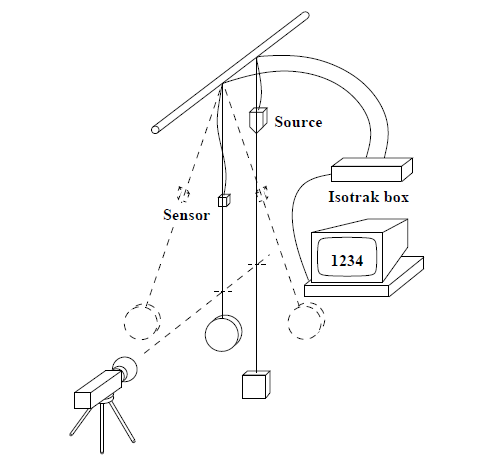
\includegraphics[scale=.6]{Figures/LiangPendulum}
		\caption{Méthode du pendule pour le calcul de la latence.}{Image tirée de \citep{liang_temporal-spatial_1991}}
		\label{fig:liang_pendulum}
	\end{figure}
	
	\par \citep{jacoby_improved_1996} utilisent également un pendule mais sans traitement vidéo a posteriori qui peut être un facteur d'imprécisions si la fréquence de capture d'image est trop basse (on risque de ne pas avoir l'image qui montre l'alignement parfait mais celle avec quelques degrés de plus ou de moins). Dans ce protocole, un ordinateur affiche une scène d'environ 1000 polygones non texturés et est relié à un système émetteur-receveur infrarouge. Le pendule coupe le rayon infrarouge à un certain point de sa course, ce qui a pour effet d'envoyer un ordre vers l'ordinateur qui doit modifier la couleur de certains de ces polygones. Un photodétecteur surveille en permanence l'écran et envoie un signal en tension lorsqu'il détecte le changement de couleur sur l'écran. Le système infrarouge et le photodétecteur sont tous deux cablés sur un oscilloscope qui permet de mesurer avec précision le temps entre leurs signaux respectifs.
	
	\par Parallèlement, il existe d'autres techniques qui ont été mises au point et qui n'impliquent pas de pendule et de mouvement oscillatoire. \citep{swindells_system_2000} génèrent un mouvement cyclique et périodique à l'aide de la table tournante d'un lecteur de vinyles. Un patch de forme ronde est placé et tracké sur la table tournante. Son mouvement est reproduit dans une scène virtuelle (Fig. \ref{fig:swindells_phonograph}). L'écart angulaire est mesuré entre le disque réel et le disque virtuel via des prises photo ou vidéo. La vitesse de rotation étant fixée et connue, on peut alors déduire le temps de latence généré par le système.
	
	\begin{figure}
		\centering
		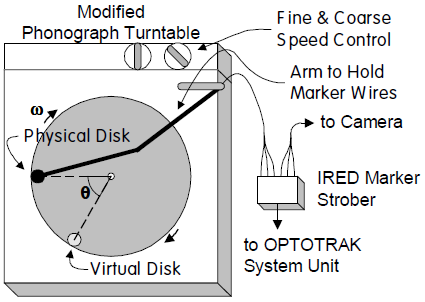
\includegraphics[scale=.75]{Figures/SwindellsPhonograph}
		\caption{Méthode de la table tournante pour le calcul de la latence.}{Image tirée de \citep{swindells_system_2000}. La position du disque physique est appliqué au disque dans la scène virtuelle. Les deux images sont superposées et on mesure l'écart angulaire entre les deux. A partir de la vitesse de rotation on peut remonter à la latence.}
		\label{fig:swindells_phonograph}
	\end{figure}
	
	\par \citep{steed_simple_2008} proposent une autre méthode de pendule tracké, annoncée plus simple que les précédentes. Une diode électroluminescente rouge est fixée à un pendule et trackée grâce à un système optique. Le mouvement de la diode rouge est reproduit en vert sur un écran placé derrière le pendule tandis qu'une caméra filme l'ensemble. A partir de la vidéo, on peut être en mesure de reproduire les sinusoïdes que décrivent les mouvements des diodes réelle et virtuelle et ainsi en déduire la latence du système en prenant le temps crête à crête.
	
	\par Si les méthodes décrites jusqu'à présent sont très abstraites par rapport au déroulement réel d'une application en VR, \citep{di_luca_new_2010} propose une technique adaptative: que ce soit pour des lunettes 3D, pour un objet quelconque ou pour un casque de Réalité Virtuelle. La méthode nécessite deux photodétecteurs: le premier placé sur l'objet à tracker et le second au niveau de l'écran qui servira à afficher l'image pour le sujet: dans le cas d'un casque, les deux photorécepteurs seront placés sur le même objet (mais à des positions différentes) alors que dans le cas d'un CAVE, les photorécepteurs seront distants (l'un sur les lunettes, l'autre au niveau d'un écran). On affiche, devant le premier photorécepteur (celui sur l'objet tracké), l'image fixe d'un gradient lumineux (un dégradé du noir vers le blanc typiquement). Si on déplace l'objet tracké dans le sens du gradient, on pourra obtenir l'équivalent de sa <<~position~>> via la valeur de luminosité qu'il mesure. De l'autre côté, le deuxième photodétecteur est dirigé vers l'écran destiné à l'utilisateur, sur lequel on affiche une nuance de gris (uniforme sur tout l'écran) en fonction des informations de tracking que l'on reçoit. En comparant le temps auquel le photorécepteur passe devant une nuance de gris donnée (en se déplaçant le long du gradient) et le temps où l'écran de l'utilisateur affiche cette même nuance de gris, on obtient la latence globale du système.
	
	\begin{figure}
		\centering
		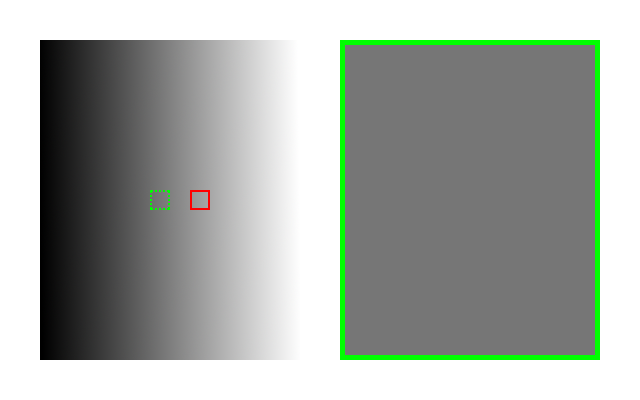
\includegraphics[scale=.5]{Figures/DiLucaGradient}
		\caption{Méthode des gradients pour le calcul de la latence.}{Le cadre rouge représente la zone réellement mesurée par le photorécepteur tandis que le grand cadre vert montre la couleur affichée par l'écran final, ce qui correspond à une <<~position~>> sur le gradient fixe représentée par le cadre vert en pointillés. La différence entre les deux petits cadres permet de calculer la latence du système.}
		\label{fig:di_luca_gradient}
	\end{figure}
	
	\par Néanmoins, les méthodes impliquant des pendules ont un défaut majeur: les 6 axes de mouvements sont autorisés, ce qui donne un mouvement avec une composante fondamentale et des petites composantes harmoniques. Ces dernières peuvent influer sur le résultat final en augmentant subrepticement l'amplitude du mouvement par rapport à la théorie. Pour minimiser ces effets indésirables, \citep{papadakis_system_2011} proposent donc une méthode similaire au plateau tournant, avec un un système limité à 3 degrés de liberté dont 2 fixés. Une rotation est générée avec un servo-moteur et contrôlée avec un encodeur, le tout relié à un oscilloscope. L'environnement virtuel lit les valeurs de l'encodeur et est programmé de telle manière que, lorsque certains seuils de rotation sont franchis, il affiche un changement graphique (un carré de couleur blanche devient noir et inversement). Une photodiode placée au niveau de l'écran surveille ce carré et renvoie un signal à l'oscilloscope en cas de changement. Le reste de la scène virtuelle est un environnement lourd en polygones (environ 140000) et soumis à des calculs de lumière complexes afin de se rapprocher des usages normaux. On relève enfin la mesure de la latence sur l'oscilloscope avec le temps entre le passage de seuil au niveau de l'encodeur, et le changement de couleur au niveau de la photodiode.
	
	\par Bien que, dans l'idéal et pour maximiser la précision dans les mesures, il faudrait utiliser un oscilloscope, nous utiliserons pour notre expérimentation une méthode par la vidéo semblable à celle proposée par \citep{steed_simple_2008}, pour mesurer la latence de nos propres systèmes ; la précision étant suffisante pour notre application (voir chapitre suivant).
	
	
\chapter{Mise en place du dispositif expérimental}
	\par On connait maintenant mieux le contexte de la latence dans la Réalité Virtuelle. On pourra donc utiliser ces connaissances pour la planification et la réalisation d'une expérimentation. Si on connait les seuils de perception et de discrimination de la latence, la variation de la performance n'est pas décrite: on sait simplement qu'elle est impactée par la latence. Il pourrait également être intéressant de se pencher sur la différence d'influence de la latence par rapport au système immersif en lui même. On fixe donc un certain nombre d'objectifs pour cette expérimentation:
	\begin{itemize}
		\item Développer un des critères prépondérant du modèle de score de réalisme.
		\item Observer l'influence de la latence sur la performance, en milieu immersif.
		\item Comparer entre deux moyens immersifs (un casque et un simulateur type CAVE).
		\item Déterminer un seuil au delà duquel l'expérience utilisateur devient trop impactée. 
	\end{itemize}
	
	\par On présente dans ce chapitre la mise en place de notre expérimentation: l'établissement du protocole pour les sujets, les techniques mises au point pour mener à bien les différentes modalités et les mesures préliminaires nécessaires au bon fonctionnement de la manipulation.
	
	\section{Tâche à effectuer}
	\par Les sujets étaient confrontés à une situation écologique, c'est à dire sensée représenter la vie <<~réelle~>>, et il leur était demandé de réaliser une tâche de tous les jours telle que regarder à des endroits précis dans le cockpit d'une voiture, pendant de courts laps de temps.
	
	\subsection{Moyens immersifs}	
	\par Un des objectifs de l'expérimentation étant de faire également une comparaison entre plusieurs moyens immersifs,	on fait passer nos sujets dans un casque de Réalité Virtuelle (un Oculus Rift) et dans un simulateur de type CAVE.
	
	\par Le CAVE est le même que pour les précédentes expérimentations: que ce soit pour le contraste et la luminance ou pour la conduite suivie de questionnaires. Les sujets sont donc assis dans un CAVE 4 faces à 1 mètre de distance de la face principale (avant). Les sujets n'étaient pas assis sur un siège de voiture comme dans nos autres expérimentations mais sur un siège normal. Ce changement est dû à plusieurs raisons: premièrement, aucune tâche de conduite n'était nécessaire, ensuite, pour garder la continuité avec la chaise de même format utilisée pendant les essais dans le casque, et enfin,  pour des facilités de manœuvre. Les sujets n'étaient donc équipés que des lunettes de stéréoscopie et d'une manette de jeu faisant office d'interface de contrôle. Du point de vue des performances graphiques, l'application utilisée pendant l'expérimentation tournait à une valeur constante de 60 images par seconde.
	
	\par La partie casque de Réalité Virtuelle s'appuyait sur un Oculus Rift de type CV1 (Commercial Version 1, voir Fig. \ref{fig:oculus_rift}). L'utilisation du casque se faisait assis à une table disposée dans un des coins du CAVE, hors de vue d'un sujet passant dans le simulateur. L'assise se faisait au moyen d'une chaise parfaitement identique à la première pour assurer une continuité entre les deux. La caméra de tracking était placée sur la table, cette dernière servant aussi pour la réponse aux différents questionnaires (voir ensuite). De cette manière, les sujets pouvaient enchainer les deux moyens immersifs sans coupure. En terme de performances, l'application était stabilisée à 90 images par seconde.
	
	\par L'environnement virtuel était commun au CAVE et au casque: le sujet était assis au volant d'une voiture (modèle <<~officiel~>> interne Renault), à l'arrêt dans un <<~paysage~>> constitué de l'intérieur des bâtiments de Renault. Le paysage était réalisé au moyen d'une photo 360 degrés pour un maximum de photo-réalisme et pour limiter le nombre de triangles à afficher dans la scène (déjà bien chargée par le modèle de la voiture). Les lumières et réflexions des miroirs étaient pré-calculées pour limiter au maximum l'impact sur le temps de calcul des images.
	
	\begin{figure}
		\centering
		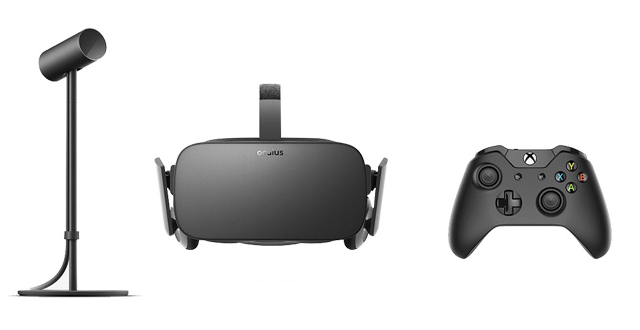
\includegraphics[scale=.65]{Figures/OculusRift}
		\caption{Oculus Rift et ses accessoires.}{De gauche à droite: la caméra permettant de tracker le casque, le casque vu de face (version CV1) et la manette de Xbox associée.}
		\label{fig:oculus_rift}
	\end{figure}
	
	\subsection{Détail de la tâche}	
	\par Une fois correctement installés dans l'environnement immersif, derrière le volant virtuel, les sujets pouvaient déclencher le début de la séquence de mesure. Il leur était alors demandé de viser visuellement des endroits précis (des <<~cibles~>>) dans la voiture, dans un ordre aléatoire, aussi rapidement et précisément que possible. La visée était aidée avec un réticule semblable à ce qui se fait dans les jeux vidéo, attaché au mouvement de la tête (voir le viseur rouge, Fig. \ref{fig:apparatus_latency}). Les cibles à viser étaient indiquées par une flèche blanche pointant une direction parmi 4 possibles (à gauche, à droite, en haut et en bas). Chaque direction de la flèche était associée à une cible: vers la gauche pour le rétroviseur gauche, vers la droite pour le rétroviseur droit, vers le haut pour le rétroviseur central et vers le bas pour la console centrale (l'écran tactile), voir Fig. \ref{fig:apparatus_latency}.
	
	\par Aussitôt que les sujets estimaient être au centre de la cible désignée, ils devaient appuyer sur un bouton (toujours le même) sur une manette de jeu (voir Fig. \ref{fig:oculus_rift}) qu'ils tenaient entre leurs mains. Chaque séquence dans le casque ou dans le CAVE était composée de 24 cibles à viser successivement (6 fois chacune des 4 cibles, mélangé aléatoirement). Les sujets devaient replacer leur réticule (et par conséquent la position de leur tête) à une position neutre après chaque visée: à l'endroit d'apparition de la flèche blanche.
	
	\par A chaque fois que les sujets appuyaient sur la manette et qu'ils étaient (par la biais du réticule) dans la cible désignée, le programme déclenchait une série de mesures (temps de passage, précision sur les axes vertical et horizontal, ...) qui sont décrites plus précisément dans la section suivante. Dans le cas d'un appui sur la manette sans cible désignée, en dehors de toute cible ou sur la mauvaise cible, rien ne se passait.
	
	\begin{figure}
		\centering
		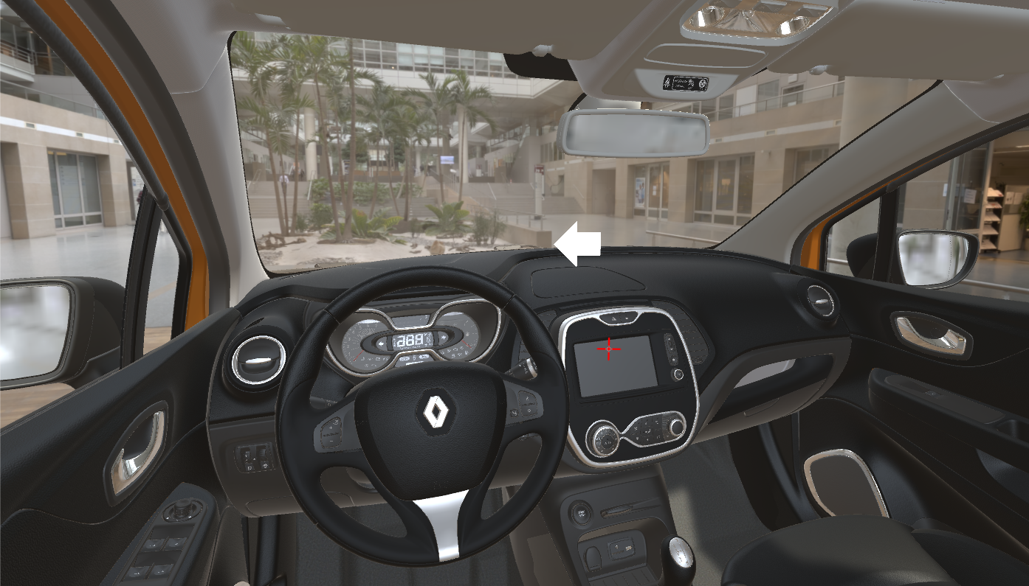
\includegraphics[scale=.9]{Figures/ExpeLatency}
		\caption{Environnement virtuel pour l'expérimentation sur la latence.}{L'image est tirée du point de vue du sujet, la flèche blanche indique la cible à viser (ici, le rétroviseur gauche) tandis que la croix rouge (le viseur) est alignée avec la direction de la tête.}
		\label{fig:apparatus_latency}
	\end{figure}
	
	\par La même séquence de 24 cibles (avec néanmoins un ordre différent puisque celui-ci était tiré aléatoirement au début de chaque séquence) était répétée 6 fois: 4 fois dans le casque et 2 fois dans le CAVE. Là encore, l'ordre de passage était mélangé aléatoirement entre les sujets pour éviter tout biais. Pour éviter de nombreux aller-retours et une re-calibration avant chaque passage, les séquences dans le casque et dans le CAVE étaient groupées: le sujet pouvait commencer aléatoirement par le casque ou par le CAVE, puis les modalités pour chaque équipement étaient vécues dans un ordre aléatoire. La différence entre chaque modalité pour le casque comme pour le CAVE était la quantité de latence globale par rapport au tracking des mouvements de la tête (d'où la manière de déplacer le réticule).
	
	\par Les deux premières modalité de latence sont évidemment, pour le CAVE et pour le casque, le fonctionnement à leur latence nominale. On ajoute ensuite, pour chacun des deux moyens immersifs, un offset de $60~ms$ de latence. La quantité de latence ajoutée a été choisie en fonction de la littérature, pour être au dessus du seuil de perception et ainsi s'assurer une influence de la latence sur les sujets. Les techniques déployées pour ajouter artificiellement de la latence sont décrites dans une section suivante (Paragraphe \ref{sec:ajout_latence_artificielle}). Les deux dernières modalité de latence sont pour le casque de Réalité Virtuelle: sa latence nominale étant bien moins élevée que celle du CAVE, on peut donc le <<~ralentir~>> jusqu'à atteindre les latences nominale, et après ajout de latence, du CAVE. On se retrouve donc avec 6 expériences différentes de latence (Tab. \ref{tab:latence_casque_cave_expe}).
	
	\begin{table}[h]	
		\centering
		\caption{Mesures de latence (en ms) pour le casque et le CAVE.}
		\label{tab:latence_casque_cave_expe}
		\begin{tabular}{c|c|l}
			\textbf{Système} & \textbf{Latence}\\
			CAVE & $160~ms$ & latence nominale\\
			CAVE & $220~ms$ & latence dégradée\\
			Oculus Rift & $45~ms$ & latence nominale\\
			Oculus Rift & $105~ms$ & latence dégradée\\
			Oculus Rift & $160~ms$ & latence niveau nominal du CAVE\\
			Oculus Rift & $220~ms$ & latence niveau dégradé du CAVE\\
		\end{tabular}
	\end{table}
	
	\par Il aura été nécessaire de faire des mesures préliminaires pour déterminer les latences nominales de nos deux système ainsi que vérifier les valeurs des offsets ajoutés. Ces mesures et la méthode mise en œuvre (inspirée des techniques vues précédemment) sont détaillées plus bas (Paragraphe \ref{sec:mesures_prelim_latence}).
	
	\subsection{Mesures}
	\par Tout au long du passage d'un sujet, un certain nombre de paramètres sont mesurés ou relevés. Certains de manière complètement transparente vis à vis du sujet et donc à priori objectives, d'autres via des questionnaires remplis au fur et à mesure de la session. C'est sur la base de ces données que l'on pourra mener des études statistiques.
	
	\par Le premier type de mesure concerne le temps global mis pour toucher l'ensemble des cibles, l'ordre des cibles, le temps par cible, et enfin, la précision relative (en valeur absolue) de la visée. Cette dernière est découpée selon l'axe horizontal (x) et l'axe vertical (y) (voir Fig. \ref{fig:x_y_precision_latency}) et est calculée en valeur absolue de manière relative à la taille de la cible: si le sujet arrive à viser précisément le centre de la cible, il obtiendra un résultat de (0,0) alors que s'il vise dans un des angles il obtiendra un résultat de 1 sur les deux axes.
	
	\begin{figure}
		\centering
		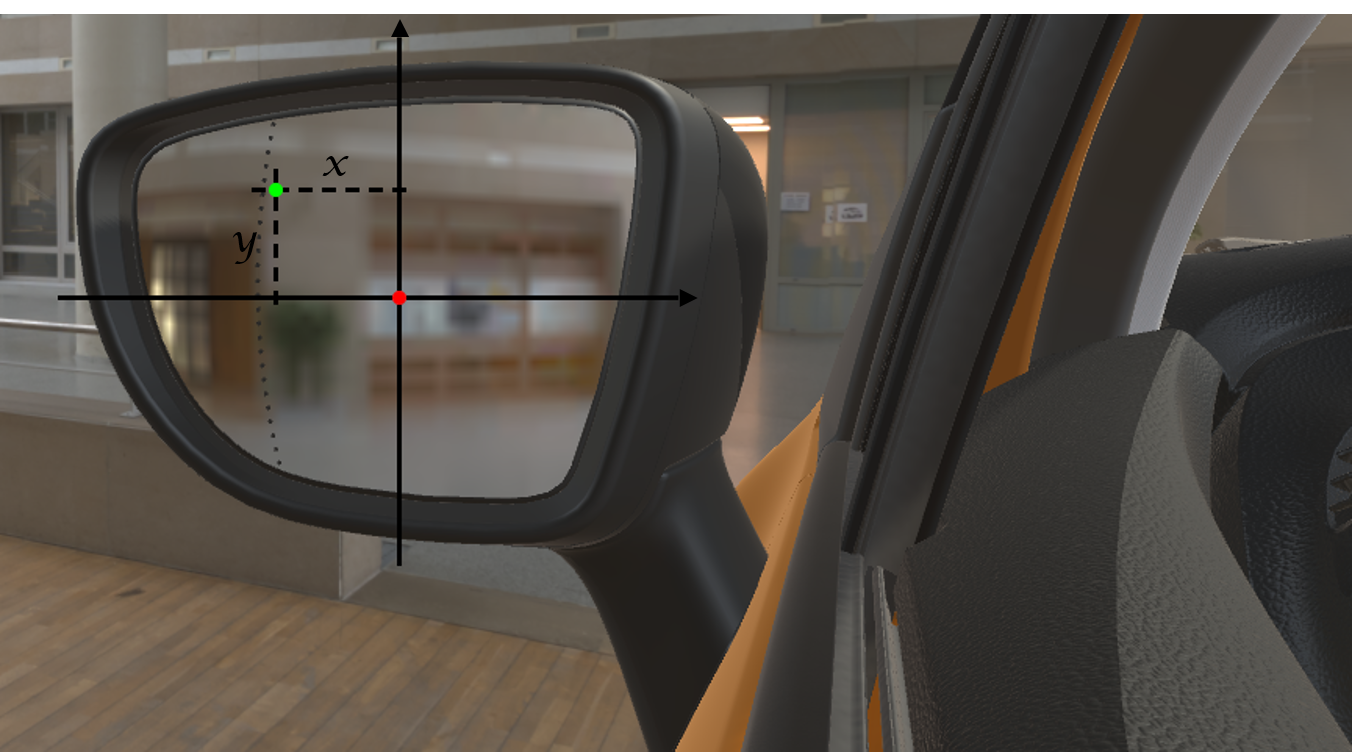
\includegraphics[scale=.65]{Figures/XYPrecision}
		\caption{Précisions en X et Y pour l'expérimentation sur la latence.}{Le point rouge correspond au centre théorique de la cible à viser (ici le rétroviseur gauche) tandis que le point vert représente le point réel que le sujet a visé.}
		\label{fig:x_y_precision_latency}
	\end{figure}
	
	\par Le sujet est également amené à remplir des questionnaires tout au long de l'expérimentation, avec notamment les questionnaires de propension à l'immersion \citep{witmer_measuring_1998}, de présence \citep{witmer_measuring_1998} et de mal du simulateur de Kennedy (SSQ). Avant de commencer l'expérimentation, tous les sujets commencent par un questionnaire de propension à l'immersion et un questionnaire de mal du simulateur, pour établir leur état <<~initial~>>. Après chaque passage dans le casque ou dans le CAVE, les sujets doivent remplir à nouveau un questionnaire de mal du simulateur. Après la meilleure condition (c'est à dire celle qui propose la latence la plus basse, la condition nominale) dans le casque, les sujets remplissent un questionnaire de présence. De même pour le CAVE. Les questionnaires utilisés étant originellement en anglais, on utilise les versions traduites en français et vérifiées par \cite{bouchard_revising_2007, bouchard_side_2009, bouchard_exploring_2011}. Ces derniers sont disponibles en annexes.
	
	\par Les questionnaires sont sous-divisés en catégories qui ne nous sont pas toutes utiles. Le questionnaire de cyber-malaise (SSQ) comporte les axes <<~nausée~>> et <<~oculomoteur~>>, que l'on conserve tous les deux car on ne se concentre pas sur un type spécifique de mal du simulateur.
	
	\par Le questionnaire de propension à l'immersion (ITQ) est divisé en 4 axes: <<~focus~>>, <<~implication~>>, <<~émotions~>> et <<~jeu~>>. On ne conserve que les questions liées aux deux premiers axes car les suivants ne sont pas cohérents avec notre expérimentation.
	
	\par Enfin, le questionnaire de présence (PQ) est divisé en 7 axes, dont deux optionnels (que l'on marquera d'une astérisque *): <<~réalisme~>>, <<~possibilité d'agir~>>, <<~qualité de l'interface~>>, <<~possibilité d'examiner~>>, <<~auto-évaluation de la performance~>>, et <<~auditif*~>>, <<~haptique*~>>. Encore une fois, on ne garde que les axes cohérents avec l'expérimentation à savoir ceux sur le réalisme, la possibilité d'agir et l'auto-évaluation de la performance.
		
	\section{Ajout de latence artificielle}
	\label{sec:ajout_latence_artificielle}
	\par L'ajout de latence artificielle a été déployé de deux manières différentes, pour le casque et le CAVE. Cet écart vient des solutions logicielles et matérielles utilisées.
	
	\subsection{Dans le casque}
	\par On utilise le SDK de SteamVR pour afficher notre environnement 3D dans le casque de Réalité Virtuelle. Celui-ci utilise des scripts qui à la fois récupèrent les données issues des capteurs (pour suivre le mouvement de la tête) et à la fois calculent les pyramides de vision et la déformation de l'image pour être amenée aux yeux à travers les lentilles. Nous avons essayé dans un premier temps de modifier directement le script de position en y insérant une temporisation entre le moment où les informations des capteurs sont prises, et le moment où elles sont appliquées. Cette méthode ne donnant pas de résultats, nous avons du contourner le problème.
	
	\par Nous avons donc créé une seconde caméra, paramétrée de manière à pouvoir afficher dans le casque, mais dont la position n'est pas mise à jour avec les informations des capteurs. En lieu et place, nous avons créé notre propre script qui prend la position et la rotation dans l'espace de la première caméra, stocke le tout pendant un temps que l'on spécifie, après lequel il applique ces données à la seconde caméra. En parallèle, on force la seconde caméra à s'afficher par dessus la première en permanence. On a donc la caméra originelle qui remplit son travail de récupération des informations des capteurs et qui suit parfaitement les mouvements de l'utilisateur mais qui n'est pas affichée, et une deuxième caméra dont on voit les images et qui calque son mouvement, avec du retard, sur la première caméra.
	
	\par Cette technique nous laisse la plus grande liberté quant au temps maximal de latence que l'on veut ajouter mais est limitée en précision par le frame rate de l'application: la récupération des informations se fait à chaque calcul d'une nouvelle image. Dans notre cas, l'application tournant à 90 images par seconde, l'imprécision moyenne était donc d'une demi-frame, soit $5~ms$. Au regard des valeurs de latence que l'on ajoute, cela implique un pourcentage d'erreur inférieur à 10\% dans la situation la plus critique.
	
	\subsection{Dans le CAVE}	
	\par Dans le cas du CAVE, la captation des mouvements de l'utilisateur se fait avec un logiciel extérieur (Dtrack 2, de A.R.T.) qui communique ensuite ses données à l'application qui transpose notre simulation en affichage immersif (MiddleVR). Dtrack permet, via des filtres, une anticipation des mouvements qui sont trackés. Si l'on peut régler la puissance de l'anticipation, on peut également lui donner des valeurs négatives, créant ainsi du retard dans les transmissions des données de position et de rotation. C'est cette méthode que l'on utilise dans le CAVE pour générer de la latence artificielle.
	
	% Figure filtre
	
	\section{Mesures préliminaires}
	\label{sec:mesures_prelim_latence}
	\par Une fois les techniques d'ajout de latence déployées, nous avons mis en œuvre, en nous inspirant de ce qui avait été fait dans la littérature et qui a été présenté précédemment, une technique pour mesurer la latence de nos systèmes de Réalité Virtuelle, en condition d'expérimentation. Cette dernière n'étant de nature psychophysique pure et ne visant pas à déterminer très précisément des seuils, nous nous accommodons d'une technique <<~moins~>> précise qu'une technique à l'oscilloscope.
	
	\par Nous avons donc opté pour un procédé filmé à grande vitesse. La mesure de la latence se faisant ensuite en analysant la vidéo image par image pour déterminer l'écart entre le début d'un mouvement et sa prise en compte et son affichage par le logiciel. On filme à 120 images par seconde avec un smartphone.
	
	\par L'objectif est donc de mesurer la latence tout en restant dans les même conditions que celles de l'expérimentation. On place donc un objet (un plan) dans l'habitacle de la voiture qui sera chargé d'afficher les variations de l'objet tracké: les lunettes de stéréoscopie pour le CAVE et le masque entier pour le casque. Ce plan se colore en vert lorsqu'il détecte que le mouvement de l'objet tracké est ascendant (c'est à dire lorsque la coordonnée sur l'axe vertical de l'objet tracké est supérieure à sa valeur de l'image précédente), et se colore en rouge lorsqu'il détecte l'inverse.
	
	\par On demande ensuite à une personne d'imprimer verticalement un mouvement sinusoïdal à l'objet tracké et on filme, avec, dans le plan, l'objet bougé et le plan changeant de couleur. On peut donc déterminer visuellement quand est ce que l'opérateur commence un mouvement ascendant ou descendant, puis compter le nombre d'image de la vidéo jusqu'au changement de couleur du plan, signifiant la prise en compte du changement. Plus le nombre d'images entre les deux marqueurs est grand, plus la latence est importante: il s'écoule $8~ms$ entre chaque image de la vidéo. On peut donc mesurer facilement la latence de nos outils, avec une précision d'une demi-image, soit $4~ms$.
	
	\par En fonctionnement dans la scène virtuelle qui sera utilisée pour l'expérimentation, on mesure une latence nominale de $45~ms$ pour le casque et de $160~ms$ pour le CAVE. La latence très élevée du simulateur vient de son architecture: les cartes graphiques et les projecteurs ont besoin d'une durée de plusieurs cycles de rafraichissement pour fonctionner, ce qui augmente la latence. Avec une architecture plus directe, avec un seul cycle de fonctionnement, la latence serait beaucoup plus basse. On a également mesuré et vérifié que les techniques pour ajouter de la latence donnaient bien les niveaux attendus: le delta de $60~ms$ pour le casque et le CAVE et les niveaux de latence équivalent à ceux du simulateur pour le casque. Les résultats de nos mesures sont synthétisés en Tab. \ref{tab:latence_casque_cave_expe}. On peut donc ainsi débuter une campagne de mesure sur des sujets, dont les résultats sont développés dans le chapitre suivant.
	
	\begin{figure}
		\centering
		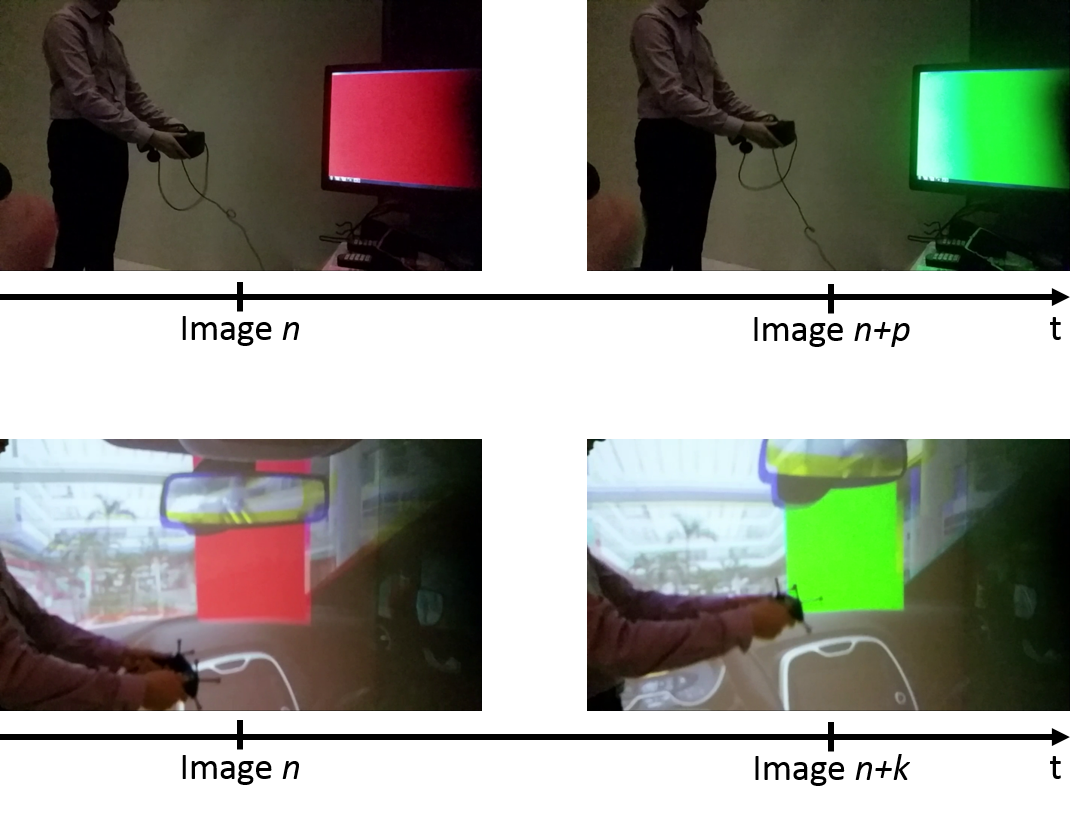
\includegraphics[scale=.8]{Figures/LatencyMeasureTechnique}
		\caption{Technique de mesure de la latence.}{On compte le nombre d'image de la vidéo ralentie entre le début du mouvement (ici, vertical ascendant) et la prise en compte du mouvement par le logiciel, signalée par le passage d'une texture du rouge au vert.}
		\label{fig:mesure_latence_video}
	\end{figure}
	
\chapter{Conclusions expérimentales}
	\par Pour notre expérimentation, nous avons réuni 32 sujets, 17 hommes et 15 femmes. 2 sujets parmi les hommes n'ont pas vu leur résultats retenus pour différentes raisons: l'un n'a pas pu faire tous les segments proposés (mal du simulateur trop élevé) tandis que l'autre fermait les yeux pour contrer ce même mal du simulateur. On termine donc avec 30 sujets ayant des données exploitables, à parité homme femme parfaite. Les sujets étaient âgés de 23 à 54 ans, avec un âge moyen de $31$ ans (écart-type: $\sigma = 11$ ans).
	
	\par On présente ici tous les résultats de l'expérimentation, et leurs implications. On traite d'abord séparément le CAVE et le casque, avant de les analyser ensembles. On met enfin en avant les enseignements que l'on peut en retirer pour le critère de latence.
	
	\section{Résultats}
	\subsection{Dans le CAVE}
	\par De manière générale, tous les résultats numériques (moyennes et écarts-types) relatif aux modalités dans le CAVE sont résumés en Table \ref{tab:resultats_cave_latence}, avec QPI: Questionnaire de propension à l'immersion, QEP: Questionnaire de présence, SSQ: Questionnaire de cyber-malaise, X et Y: précision sur les axes respectifs et t: temps de complétion.
	
	\begin{table}[h]	
		\centering
		\caption{Expérimentation latence: résultats moyens et écarts-types dans le CAVE.}
		\label{tab:resultats_cave_latence}
		\begin{tabular}{c|c|c|c|c|c|c}
			\textbf{Latence} & \textbf{QPI} & \textbf{QEP} & \textbf{SSQ} & \textbf{X} & \textbf{Y} & \textbf{t}\\ \hline			
			$160~ms$ & $43.83$ & $67.50$ & $3.37 \pm 3.25$ & $0.18 \pm 0.07$ & $0.17 \pm 0.08$ & $101.49 \pm 14.31$\\
			$220~ms$ & $\pm 7.50$ & $\pm 11.33$ & $4.60 \pm 4.91$ & $0.22 \pm 0.09$ & $0.19 \pm 0.10$ & $128.61 \pm 24.79$\\
		\end{tabular}
	\end{table}
	
	\par Initialement, les sujets répondent à un questionnaire de propension à l'immersion (moyenne des réponses: $43.83$).	Après leur passage à la condition nominale du CAVE, les sujets répondent également à un questionnaire de présence (moyenne des réponses: $67.50 \pm 11.33$, Fig. \ref{fig:itq_pq}). Il ne semble pas exister ($p = 0.07$) de corrélation statistique\footnote{Méthode: Corrélation de Pearson, 28 degrés de liberté, $Qobs = 1.91$.} entre les deux qui nous permettrait de prévoir le degré d'immersion d'un sujet sur la base d'un QPI.
	
	\par A l'issue de chaque passage dans le CAVE, en condition nominale et en condition dégradée de latence, les sujets ont répondu à un questionnaire d'auto-évaluation du cyber-malaise. Celui-ci donne des valeurs moyennes de respectivement $3.37$ pour la modalité sans latence ajoutée, et de $4.60$ pour la modalité avec latence ; soit une augmentation de $36.5\%$ du cyber-malaise avec la latence. Il existe une corrélation statistique\footnote{Méthode: Corrélation de Pearson, 28 degrés de liberté, $Qobs = 4.08$.} ($p = 0.0003$) positive-forte ($\rho = 0.61$) entre les deux jeux de valeurs: les sujets les plus malades dans la modalité la plus faible en latence, l'étaient encore plus avec l'augmentation de la latence.
	
	\par Dans le cas du CAVE sans latence ajoutée (Fig. \ref{fig:cave_precision} et Table \ref{tab:resultats_cave_latence}), la précision relative sur les deux axes (horizontal et vertical) est quasiment la même ($0.18$ contre $0.17$). Cet écart s'accentue néanmoins lorsque la latence augmente avec des valeurs moyennes de $0.22$ et de $0.19$ pour les axes horizontal et vertical respectivement. Le temps de complétion (Fig. \ref{fig:cave_completion_time} et Table \ref{tab:resultats_cave_latence}) est lui beaucoup plus sensible au changement de latence avec une valeur moyenne entre les sujets qui passe de $101.49~s$ à $128.61~s$ pour réaliser l'ensemble de la tâche.

	\begin{figure}
		\centering
		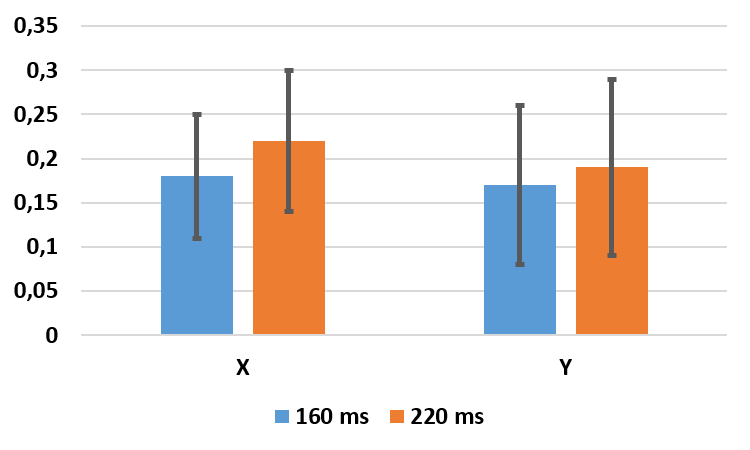
\includegraphics[width=0.8\linewidth]{Figures/CavePrecisionResults.png}
		\caption{Précision moyenne sur x et sur y dans le CAVE, en fonction de la latence.}
		\label{fig:cave_precision}
	\end{figure}
	
	\begin{figure}
		\centering
		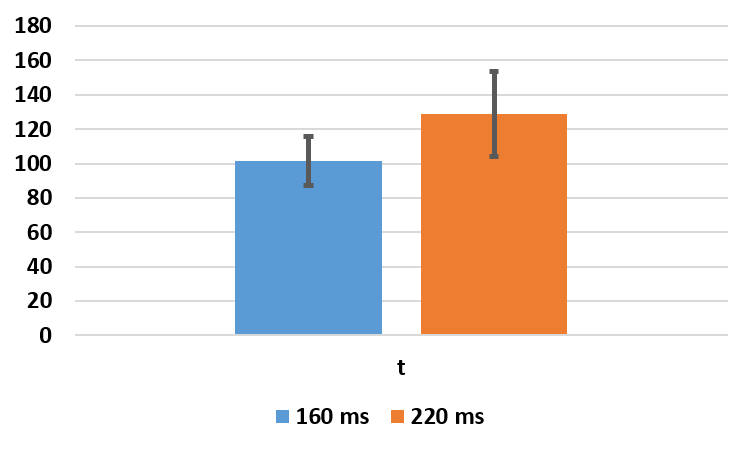
\includegraphics[width=0.8\linewidth]{Figures/CaveCompletionTimeResults.png}
		\caption{Temps de complétion moyens dans le CAVE, en fonction de la latence.}
		\label{fig:cave_completion_time}
	\end{figure}
	
	\par Du point de vue statistique, en utilisant un test de Student pour échantillons appariés (29 degrés de liberté), on montre que la latence influence la performance de manière globale ; que ce soit pour la précision sur l'axe horizontal ($p = 0.00009$), la précision sur l'axe vertical ($p = 0.015$) ou le temps de complétion ($p = 3 \times 10^{-11}$). Néanmoins, le mal du simulateur échoue au test statistique avec une p-value de $p = 0.099$. Si les sujets sont gênés par l'évolution de la latence pour viser le centre des cibles, ils sont nettement moins perturbés et ne deviennent pas significativement plus malades.
	
	\par Dans l'explication de ces résultats, un paramètre dont il faut tenir compte est le critère de vitesse qui a été demandé pour passer l'ensemble des cibles. Maintenir un rythme élevé pendant l'expérience implique moins de soin apporté à la précision de la visée. Par conséquent, nos résultats montrent une moins bonne précision par rapport à ce qui aurait pu être atteint si l'ordre aurait été de simplement viser le centre des cibles. Dans le cas actuel du CAVE, la précision moyenne des sujets au-dessus de la médiane du temps d'achèvement (dans la configuration de latence plus élevée) est supérieure à la précision moyenne des sujets en dessous de la médiane du temps d'achèvement : 0,26 contre 0,21 sur l'axe horizontal et 0,23 contre 0,16 sur l'axe vertical. Par conséquent, outre le temps d'interaction, un rythme plus élevé dans des conditions de latence plus élevées entraîne une plus grande imprécision. 

	\par Ces deux modalités dans le CAVE ne sont évidemment pas suffisantes pour tirer des conclusions définitives et il nous reste à explorer les résultats propres au casque qui, qui plus est, bénéficie de niveaux de latence bien moins élevés, mais aussi la comparaison entre les systèmes immersifs, à latence équivalente.
	
	\subsection{Dans le casque}
	\par De même que précédemment, tous les résultats numériques (moyennes et écarts-types) relatif aux modalités dans le casque sont résumés en Table \ref{tab:resultats_casque_latence}. On constate une influence statistique\footnote{Méthode: test de Friedman, 3 paramètres.} de la latence sur le cyber-malaise ($p < 2 \times 10^{-7}$) et sur toutes les modalités de la performance: précision sur l'axe horizontal ($p = 0.034$), sur l'axe vertical ($p = 0.024$), et le temps de complétion ($p < 8 \times 10^{-10}$).
	
	\begin{table}[h]	
		\centering
		\caption{Expérimentation latence: résultats moyens et écarts-types dans le casque.}
		\label{tab:resultats_casque_latence}
		\begin{tabular}{c|c|c|c|c|c|c}
			\textbf{Latence} & \textbf{QPI} & \textbf{QEP} & \textbf{SSQ} & \textbf{X} & \textbf{Y} & \textbf{t}\\ \hline			
			$45~ms$ & & & $3.33 \pm 3.27$ & $0.17 \pm 0.07$ & $0.15 \pm 0.09$ & $87.74 \pm 10.40$\\
			$105~ms$ & $43.83$ & $70.07$ & $4.60 \pm 3.68$ & $0.17 \pm 0.06$ & $0.18 \pm 0.10$ & $92.85 \pm 10.58$\\			
			$160~ms$ & $\pm 7.50$ & $\pm 10.83$ & $6.23 \pm 5.55$ & $0.17 \pm 0.07$ & $0.17 \pm 0.08$ & $94.73 \pm 11.64$\\
			$220~ms$ & & & $7.40 \pm 5.62$ & $0.19 \pm 0.08$ & $0.18 \pm 0.09$ & $98.37 \pm 11.36$\\
		\end{tabular}
	\end{table}
	
	\par Là encore, après leur passage à la condition nominale de latence, les sujets répondent à un questionnaire de présence (moyenne des réponses: $70.07 \pm 10.83$, Fig. \ref{fig:itq_pq}). On compare ces résultats à ceux du questionnaire de propension à l'immersion initialement rempli. Il ne semble là non plus pas exister ($p = 0.31$) de corrélation statistique\footnote{Méthode: Corrélation de Pearson, 28 degrés de liberté, $Qobs = 1.03$.} entre les deux.
	
	\par On s'intéresse ensuite à la comparaison deux à deux des conditions de latence dans le casque: l'éventail de niveaux de latence étant plus large, on pourra déterminer plus précisément le comportement de la performance en fonction de l'évolution de la latence. Tous les tests réalisés le sont avec la méthode du test de Student pour échantillons appariés (29 degrés de liberté).
	
	\par Du point de vue de la précision horizontale, la latence n'a statistiquement d'effet ($p = 0.043$) qu'à partir de la 3ème et dernière comparaison deux à deux: entre 105 et 160~ms de latence ajoutée. Les autres confrontations (passage de 0 à 60~ms de latence ajoutée et passage de 60 à 105~ms) ne présentent aucun résultat statistique ($p = 0.90$ et $p = 0.23$ respectivement). On constate néanmoins des différences sur les résultats moyens, à partir de la 3ème décimale.
	
	\par Pour la précision verticale, la tendance est inverse: statistiquement, la latence a un effet dès la première comparaison ($p = 0.0004$) puis cesse ($p = 0.27$ et $p = 0.20$ pour les deux dernières comparaisons). Il semblerait alors que la performance de visée, dans ce cas particulier de visée rapide avec le mouvement de la tête, varie non-linéairement mais par effet de palier. Les deux mouvements, horizontal et vertical, semblent ne pas avoir la même sensibilité: le premier possède son palier aux alentours des 100~ms de latence ajoutée, tandis que le second se situe autour de 60~ms ajoutées.
	
	\begin{figure}
		\centering
		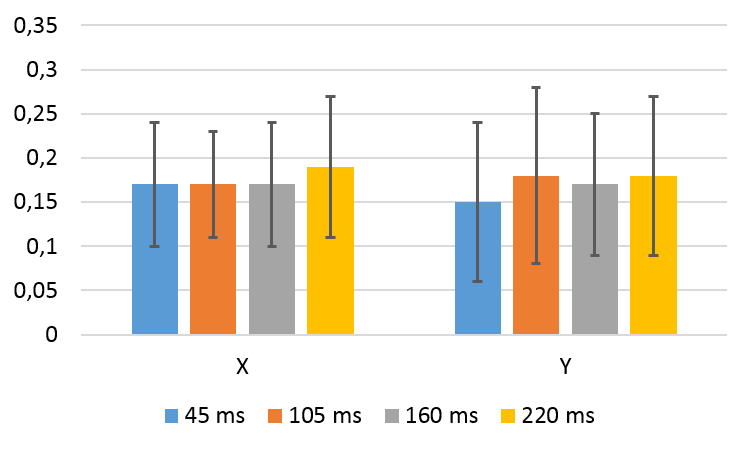
\includegraphics[width=0.8\linewidth]{Figures/CasquePrecisionResults.png}
		\caption{Précision moyenne sur x et sur y dans le casque, en fonction de la latence.}
		\label{fig:casque_precision}
	\end{figure}
	
	\par Ensuite, le temps de complétion montre une influence statistique de la latence plus erratique que la précision avec des tests validés pour la première ($p = 0.0003$) et la troisième ($p = 0.005$) comparaison, mais pas pour la deuxième ($p = 0.26$).
	
	\begin{figure}
		\centering
		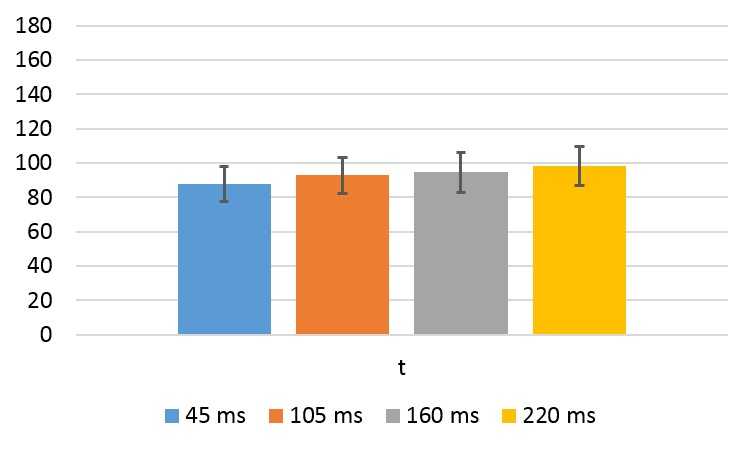
\includegraphics[width=0.8\linewidth]{Figures/CasqueCompletionTimeResults.png}
		\caption{Temps de complétion moyens dans le casque, en fonction de la latence.}
		\label{fig:casque_completion_time}
	\end{figure}
	
	
	\par Enfin, on constate un comportement différent des mesures de précision pour l'évolution du cyber-malaise: ce dernier semble évoluer graduellement en fonction de la latence, là où dans le casque on ne relevait pas d'influence statistique, toutes les confrontations deux à deux présentent des résultats positifs: $p = 0.014$ pour le passage de 0 à 60~ms ajoutées, $p = 0.036$ pour le passage de 60 à 105~ms et $p = 0.067$ pour le dernier passage, bien que la corrélation soit plus faible. Numériquement, on constate une évolution de 38 et 35\% dans les deux premiers cas, puis une augmentation de 19\% à la fin.
	
	\par Plus la vitesse des mouvements de la tête est élevée, plus la latence influence l'expérience de l'utilisateur, tant au niveau de la dégradation de la précision que de l'augmentation du mal des simulateurs. Les sujets étaient confrontés à un choix : soit ils ralentissaient leurs mouvements pour augmenter la précision, soit ils gardaient un bon rythme au détriment de la précision et du mal du simulateur. Les sujets semblent développer leur propre stratégie pour contrer le décalage de la latence, en se basant sur le niveau de cette dernière. Par conséquent, pour assurer la meilleure expérience utilisateur et minimiser le cyber-malaise, il peut être conseillé de suggérer des mouvements petits et lents aux utilisateurs quotidiens des techniques d'immersion.	
	
	\par Maintenant que l'on a détaillé les résultats propres à chaque système et à chaque niveau de latence, on s'intéresse à comparer les systèmes entre eux, lorsqu'ils ont le même niveau de latence et lorsque la latence varie de la même quantité. Au delà des valeurs de performance, on s'intéresse également aux valeurs de présence et de cyber-malaise.
	
	\subsection{Analyse croisée}
	\par Tous les tests statistiques présentés dans cette partie ont été réalisé avec la méthode du test de Student pour échantillons appariés (29 paramètres).	
	
	\par La première comparaison concerne la troisième modalité du casque et la première du CAVE. Dans cette configuration, les deux dispositifs offrent la même quantité de latence ($160~ms$). Confronter les résultats de nos sujets reviendra alors à regarder l'influence du dispositif immersif sur la tâche à réaliser. Du côté de la précision, on ne trouve aucun résultat statistique ($p = 0.41$ pour l'axe horizontal, $p = 0.79$ pour l'axe vertical) venant étayer l'hypothèse d'une influence du système immersif. Néanmoins, l'influence du changement de système est statistiquement avérée dans le cas du temps de complétion ($p = 0.0006$) avec une augmentation de $7\%$ du temps total nécessaire pour viser les 24 cibles dans le CAVE et dans le cas du cyber-malaise ($p = 0.001$) avec une augmentation de $85\%$ lorsque l'on passe dans le casque !
	
	\par Dans le cas du casque et du simulateur à 220~ms de latence totale, l'influence statistique ($p = 10^{-10}$) du changement de système sur le temps de complétion est corrélée avec une variation encore plus forte: les sujets sont $30\%$ plus lents pour terminer la séquence de visée dans le CAVE, par rapport au casque. On retrouve encore une fois une influence statistique ($p = 0.015$) sur le mal du simulateur avec une valeur moyenne supérieure de $60\%$ dans le casque par rapport au CAVE. A la différence de la précédente comparaison, il existe cette fois un lien statistique entre le changement de système et la précision de visée sur l'axe horizontal ($p = 0.0006$) avec une valeur $16\%$ plus grande dans le cas du CAVE. L'influence sur la précision sur l'axe vertical est elle toujours non vérifiée par les tests ($p = 0.49$).
	
	\par Ensuite, on compare encore les deux systèmes immersifs, mais cette fois seulement en terme de variation de performance lorsque l'on augmente la latence de 60~ms. Les moyennes de ces variations sont résumées en Table \ref{tab:resultats_delta_casque_cave}. A l'instar de la comparaison casque/CAVE en conditions de latence dégradées, on observe une influence statistique du changement de système combiné à une augmentation de latence de 60~ms sur deux des trois modalités de la performance: sur la précision horizontale ($p = 0.007$) et sur le temps de complétion ($p = 6 \times 10^{-9}$). Cela revient à dire que lorsque l'on change de système, du casque au CAVE, en augmentant la latence, la performance est deux fois perdante: d'abord de par le changement de système, mais également par le changement de latence (plus encore que simplement par un changement de latence).
	
	\begin{table}[h]	
		\centering
		\caption{Expérimentation latence: résultats moyens et écarts-types dans le casque.}
		\label{tab:resultats_delta_casque_cave}
		\begin{tabular}{c|c|c|c|c}
			& $\Delta_{60}X$ & $\Delta_{60}~Y$ & $\Delta_{60}~t$ & $\Delta_{60}~SSQ$\\ \hline
			Casque & 0.001 & 0.029 & 5.11 & 1.27\\
			CAVE & 0.039 & 0.06 & 27.15 & 1.23\\
		\end{tabular}
	\end{table}
	
	\par On observe une forte augmentation des valeurs de cyber-malaise entre toutes les configurations (environ 120\% entre les deux modalités dans le CAVE ou les deux cas extrêmes dans le casque, par exemple). Il est à noter que les valeurs moyennes de mal du simulateur pour les versions les plus dégradées en latence sont fortement influencées par des valeurs de cyber-malaise très élevées pour quelques sujets. Cela s'explique par la contribution, en plus du conflit classique vergence-accommodation, du conflit visio-vestibulaire: plus la latence est grande, plus la disparité entre la vision et la conscience du mouvement par le système vestibulaire est importante et donc le mal du simulateur.	
	
	\par Dans le cas du casque, l'effet du conflit visio-vestibulaire est amplifié: les sujets ne voient pas leur corps. Selon nous, ce problème reste le principal facteur de mal du simulateur dans le casque, et la raison de la relative tranquillité dans le CAVE. Dans le simulateur, lorsque l'on tourne la tête, si l'image bouge avec du retard, le cerveau peut se raccrocher au fait d'avoir quand même vu le corps <<~bouger~>> (lorsque l'on tourne la tête à droite, si l'on fait abstraction de l'environnement, cela revient à garder la tête fixe en faisant tourner le corps vers la gauche). Le cerveau peut décréter qu'une partie des informations visuelles est incohérente et peut s'en protéger. Dans le casque, néanmoins, le flux visuel est entièrement remplacé et lorsque l'on bouge la tête, on ne peut se référer qu'à nos centrales inertielles et l'image ayant du retard. Le cerveau ne peut pas alors déjuger cette dernière, et le mal du simulateur est plus important.
	
	\par Enfin, si on a déjà vu dans les deux sections précédentes qu'il ne semble pas être possible d'extrapoler la présence dans le casque ou dans le CAVE à partir de la propension à l'immersion (Fig. \ref{fig:itq_pq}), on vérifie néanmoins l'existence d'une corrélation\footnote{Méthode: Corrélation de Pearson, 28 degrés de liberté.} négative-forte entre la présence et le cyber-malaise vérifiée, pour les deux moyens immersifs (pour le CAVE: $p = 0.022$ avec $\rho = -0.42$ ; pour le casque: $p = 0.030$ avec $\rho = -0.40$). Bien que cela puisse sembler évident, on a la confirmation que lorsque la présence augmente, le mal du simulateur diminue, et inversement.
	
	\begin{figure}
		\centering
		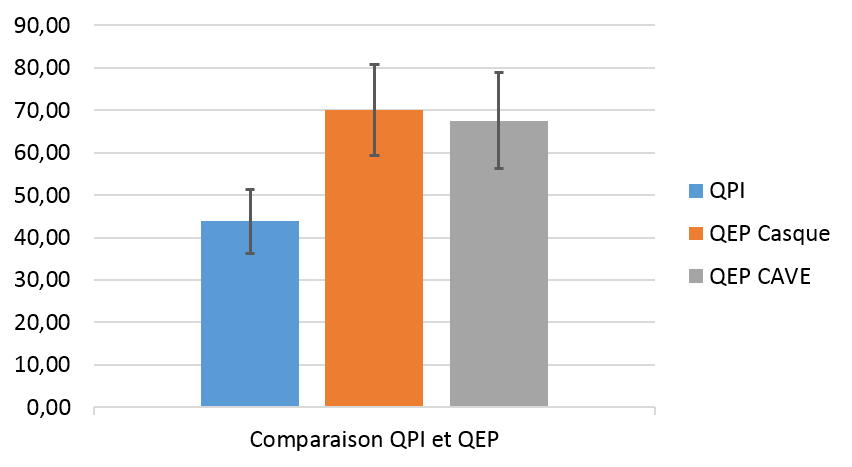
\includegraphics[width=0.8\linewidth]{Figures/ITQvPQ.png}
		\caption{Scores moyens des questionnaires de propension à l'immersion (QPI) et de présence (QEP).}
		\label{fig:itq_pq}
	\end{figure}
	
	\par Nos résultats montrent une influence statistique de la latence sur la précision. Lorsque la latence augmente, les sujets sont plus imprécis sur les mouvements latéraux que sur les mouvements verticaux. La différence entre les deux axes s'explique par la plus grande amplitude de mouvement nécessaire pour atteindre les cibles gauche et droite (miroirs gauche et droit, entre 40 et 60 degrés) par rapport à l'amplitude nécessaire pour atteindre les cibles supérieure et inférieure (miroir central et affichage central, 15 degrés). Un mouvement plus grand signifie un temps d'interaction plus long avec la latence et donc une plus grande imprécision.
	
	\section{Apport au score de réalisme}
	\par On possède désormais un certain nombre de clefs supplémentaires pour la compréhension de la relation entre la latence et l'expérience utilisateur en immersion ; au minimum du point de vue d'une tâche relativement cohérente avec celles que l'on effectue réellement. Outre les seuils de perception de la latence que l'on a vu en introduction de cette partie expérimentale, des valeurs de latence semble se dégager.
	
	\par Par rapport au fonctionnement de notre système de notation, il semble difficile de ne pas attribuer la note maximale au seuil de perception de la latence, à savoir $15~ms$. De notre expérimentation, deux seuils de performance semblaient se dégager grâce aux casques: un premier relatif aux mouvements horizontaux entre 105 et 106~ms de latence ajoutée, et un deuxième, pour les mouvements verticaux, plus sensible, entre 0 et 60~ms de latence ajoutée. De part la valeur nominale de latence du casque, le seuil le plus critique est donc pour une latence totale d'environ 105~ms. C'est la valeur que nous retiendrons pour la performance standard dans notre notation.
	
	\par Néanmoins, notre expérimentation n'a pas permis de mettre en avant un seuil limite au delà duquel la tâche n'était plus réalisable, ce qui complique l'attribution d'une note minimale au critère de latence. En première approche, il peut toutefois être envisagé de l'associer à une latence qui tend vers l'infini.